\documentclass[openany,overnay,a4paper, twoside, 12pt]{book}
\usepackage{graphicx}
\usepackage[utf8]{inputenc}
\usepackage[noindentafter]{titlesec}
\usepackage{wrapfig}
\usepackage{pdfpages}
\usepackage[document]{ragged2e} %para poder justificar el texto
\usepackage[a4paper,width=150mm,top=25mm,bottom=25mm,bindingoffset=10mm]{geometry} %igualar los margenes de las paginas pares e impares
\usepackage{hyperref} % ESTO HACE QUE EL INDICE TENGA ENLACES A LOS CAPITULOS
\renewcommand{\contentsname}{Índice} %Cambio el nombre de Content a Índice


\title{PLAN DE EMPRESA\\
\\\\\
\newline
\newline
\newline

\includegraphics[scale = 0.6]{imagenes/lixboo.png}}
%Añado la imagen justo antes en el titulo
\setlength{\parindent}{6.5ex} 




\author{
    Carcasona, Héctor\\
    Co-founder\\
    IES Ítaca\\
    6658hcarcasona@e-itaca.es
  \and
    Herrero, María\\
   Co-founder\\
    IES Ítaca\\
    0224mherrero@e-itaca.es}
\date{January 2022}
\pagestyle{plain} %Para que los numeros de página aparezcan siempre en medio 
\begin{document}
\let\cleardoublepage\clearpage %Para evitar que se cree una página vacia (Valdrá solo con uno de esos comandos???)

\maketitle
\tableofcontents %Creo el indice
\setcounter{chapter}{1}%Cambiamos el numero del capitulo
%%%%%%%%%%%%%%%%%%%%%%%%%%%%%%%%%%%
%%%%%%%	FALTA INDICE DE IMAGENES
%%%%%%%%%%%%%%%%%%%%%%%%%%%%%%%%%%%%
\chapter*{Tema 1. Empresa e iniciativa emprendedora}
\addcontentsline{toc}{chapter}{Tema 1. Empresa e iniciativa emprendedora}
%AÑADO CAPITULOS EN EL INDICE. HAY QUE PONERLO DESPUES DE CADA CAPITULO



\justifying %justifica el texto de todo el documento
\section{Actividad}
La idea de negocio va a consistir principalmente en el alquiler de libros electrónicos, de forma que nuestros clientes tengan que estar suscritos en nuestra biblioteca en línea, es decir, a través de nuestra página web. A parte, la propuesta de valor o factor diferenciador respecto a la competencia, será un tratamiento personalizado a los clientes, descubriendo y proponiendo nuevas lecturas.

\section{Clientes}
El servicio que se va a ofrecer está dirigido principalmente a aquellos lectores que prefieren los libros electrónicos y además les guste leer varios libros a la vez sin necesidad de llevarlos todos encima de forma física.

\section{Necesidad que cubre}
La necesidad que intenta cubrir la empresa, es la posibilidad de tener acceso a todos los libros que los clientes deseen mediante únicamente un clic. Además, en ocasiones, puede resultar difícil decidir qué libro escoger, lo que para evitar esa pérdida de tiempo y del dinero que supone comprarse un libro nuevo, la empresa también propondrá a los clientes unas posibles nuevas lecturas, conforme a sus gustos.

\section{Propuesta de valor}
La propuesta de valor de la empresa será, a parte de ofrecer un catalogo más asequible que la competencia, poder tener recomendaciones personalizadas basadas en tus lecturas. 

\section{Objetivo a 1 año}
El objetivo de futuro a un año no es más que cubrir la inversión inicial, incluyendo todos los gastos que se hayan generado a lo largo del primer año. Para la financiación de esta inversión, se consideran dos fuentes de financiación distintas: con fondos propios o de forma mixta, utilizando menos recursos propios y pidiendo financiación ajena en forma de préstamo. Por tanto, para elegir la mejor opción se sopesará cuál de todas las entidades financieras existentes ofrecen mejores condiciones.

\setcounter{chapter}{2} %Cambiamos el numero del capitulo
\chapter*{Tema 2. El mercado}
\addcontentsline{toc}{chapter}{Tema 2. El mercado}

\setcounter{section}{0}
\section{Cuota de mercado}

Después de realizar un estudio acerca de la cuota de mercado, se valoró que ya existían algunas empresas de este tipo, las cuales podrían convertirse en potenciales competidoras. Por lo tanto, nos encontramos en un mercado de oligopolio sin pacto.

\section{Estructura del mercado y canales de distribución}
La estructura del mercado se va a dividir en lo siguiente
\begin{itemize}
\item Fabricantes de bienes y empresas de servicios. La empresa tendrá como proveedores a las distintas editoriales existentes a nivel nacional.
\item Intermediarios o canales de distribución. La empresa únicamente contará con el fabricante.
\item Prescriptores. La empresa pactará colaboraciones con personalidades destacadas de la escena literaria actual para publicitar la imagen de la empresa.
\item Consumidores. Los demandantes del servicio que ofrece la empresa.
\end{itemize}




\section{Monopolio y oligopolio}
Se ha valorado que la cuota de mercado de la empresa se va a encontrar en un oligopolio sin pacto, ya que, existen pocas empresas competidoras, entre las más fuertes nos podemos encontrar con Amazon. Debido a esto, la empresa necesitará una gran cantidad de inversión inicial.

\section{Segmentos del mercado}
A la hora de pensar qué clientes son los que pueden necesitar o comprar el servicio. En función de los criterios de segmentación, diferenciaremos:
\begin{itemize}
\item Demográficos: Gente joven, dispuesta a usar nuevas tecnologías.
\item Económicos: Al ser los libros electrónicos mucho más baratos que los físicos, el servicio favorece a las personas con menos recursos, aunque debido a otros factores las clases más altas no quedan excluidas. 
\item Gustos: personas a las que les guste leer y no sepan qué leer en cierto momento.
\item Psicológicos: gente más innovadora y que no sean muy tradicionales.
\end{itemize}
El principal elemento diferenciador respecto a la competencia será, además de la competitividad en cuanto a precios, poder ofrecer una lista de libros que puedan interesar a los clientes.
\section{Estudio de mercado: Los clientes}
Nos interesa conocer el tipo de clientes potenciales que puedan hacer uso del servicio que ofrece Lixboo, es por eso que hemos realizado un estudio de mercado. En primer lugar, hemos hecho una encuesta, la cual aparecerá como Anexo 1, los resultados de esta encuesta son los siguientes:
\begin{figure}[h]
\centering
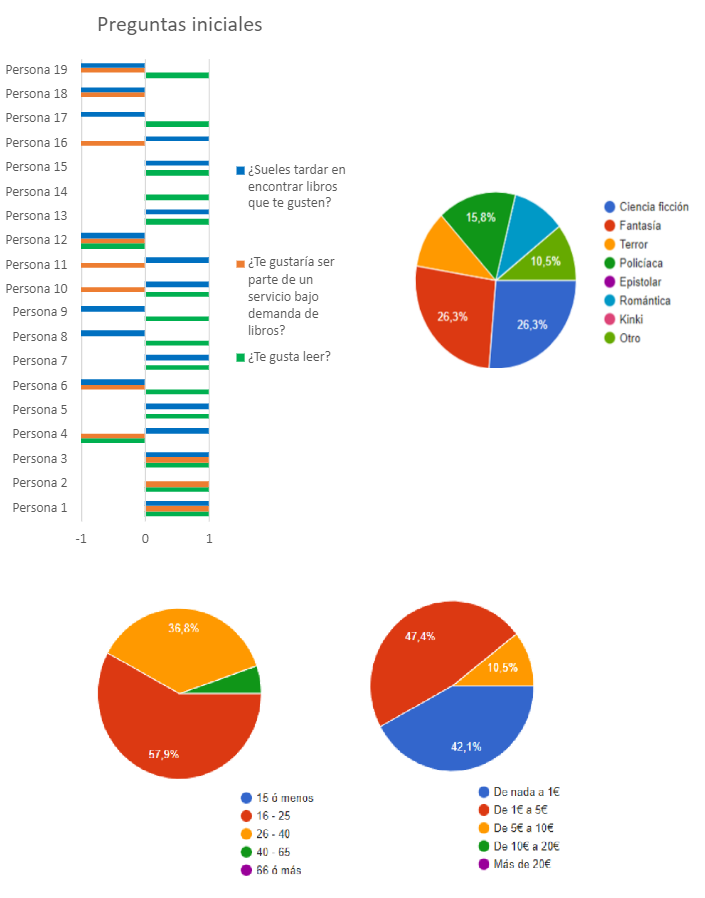
\includegraphics[scale = 0.6]{imagenes/encuesta_1.png}
\renewcommand{\figurename}{Resultado de encuesta}
\renewcommand{\figurename}{Fuente}
\caption{Propia}
\end{figure}


Tal y como se observa, los resultados obtenidos indican, que los clientes potenciales de Lixboo, serán aquellos que les guste leer (14 personas de los encuestados han votado que les gusta bastante). Algunos de ellos se han planteado en alguna ocasiones formar parte de un servicio bajo demanda. Por otro lado, 10 personas de las encuestadas afirman que les cuesta encontrar libros de su gusto. Por ello se ofrecerá un servicio  de alquiler de libros electrónicos, de forma que los clientes tengan que estar suscritos en la biblioteca biblioteca en línea. \\Además Lixboo realizará un tratamiento personalizado a los clientes, descubriendo y proponiendo nuevas lecturas.
\setcounter{chapter}{3} %Cambiamos el numero del capitulo
\chapter*{Tema 3. El entorno}
\addcontentsline{toc}{chapter}{Tema 3. El entorno}
\setcounter{section}{0}
\section{Entorno General}
\subsection{Análisis PEST}
\begin{figure}[h]
\centering

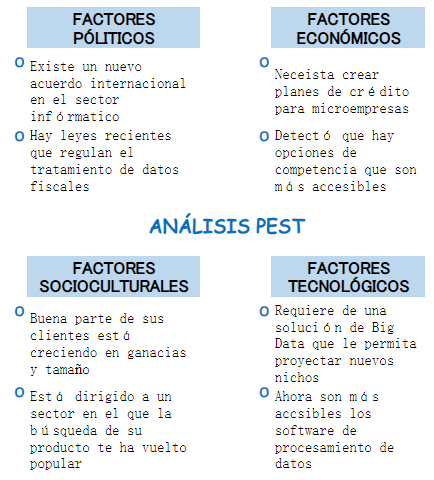
\includegraphics[scale = 0.7]{imagenes/PEST.png}
\renewcommand{\figurename}{Análisis PEST}
\renewcommand{\thefigure}{}
\caption{\textit{Factores Político-Legales, Económicos, Socioculturales, Tecnológicos}}
\renewcommand{\figurename}{Fuente}
\caption{Propia}
\end{figure}
\section{Entorno Específico}
\subsection{Grado de competencia entre las empresas actuales}
Consecuencias para la empresa
\begin{itemize}
\item Entre las grandes competidoras de la empresa se encuentran Amazon y la Casa del Libro.
\item Económicos: Al ser los libros electrónicos mucho más baratos que los físicos, el servicio favorece a las personas con menos recursos, aunque debido a otros factores las clases más altas no quedan excluidas. 
\item Gustos: personas a las que les guste leer y no sepan qué leer en cierto momento.
\item Psicológicos: gente más innovadora y que no sean muy tradicionales.
\end{itemize}
\subsection{Posibilidad de entrada de futuros competidores}
Consecuencias para la empresa:
\begin{itemize}
\item Al ser un oligopolio, será necesario la realización de una gran inversión.
\item Al principio será difícil diferenciarse o exponer el factor diferenciador de la empresa respecto al resto. 
\item La entrada de cualquier nueva empresa en un mercado supone el cumplimiento de una serie de requisitos legales.
\end{itemize}
\subsection{Las mejores de la competencia}
Los principales competidores de la empresa serán Amazon y la Casa del Libro. Ambas comparten puntos fuertes y débiles. Un resumen de estos puntos es:
\textbf{Puntos fuertes} %hay que poner en negrita o algo
\begin{itemize}
\item Son empresas bastante conocidas por los clientes reales y potenciales, en otras palabras, están asentadas en el mercado.
\item Tienen bajos costes por su gran volumen de negocio.
\item Por ejemplo, Amazon aprovecha su modelo de “Amazon Prime” para hacer competencia desleal. Además, utiliza su posicionamiento en el mercado para hacer autopromoción de sus demás servicios, como puede ser la página “Iberlibro” o su servicio de libros electrónicos.
\end{itemize}
\textbf{Puntos débiles} %hay que poner en negrita o algo
\begin{itemize}
\item No ofrecen el principal factor diferenciador que tiene la empresa: la recomendación de libros en función de las lecturas anteriores de nuestros clientes y de su modelo de usuario.
\item Estos competidores se centran en una segmentación concentrada y apenas diferencian entre sus tipos de clientes.
\item Por ejemplo, Amazon aprovecha su modelo de “Amazon Prime” para hacer competencia desleal. Además, utiliza su posicionamiento en el mercado para hacer autopromoción de sus demás servicios, como puede ser la página “Iberlibro” o su servicio de libros electrónicos.
\end{itemize}
\newpage
\section{DAFO y CAME} 

\begin{figure}[h]
\centering

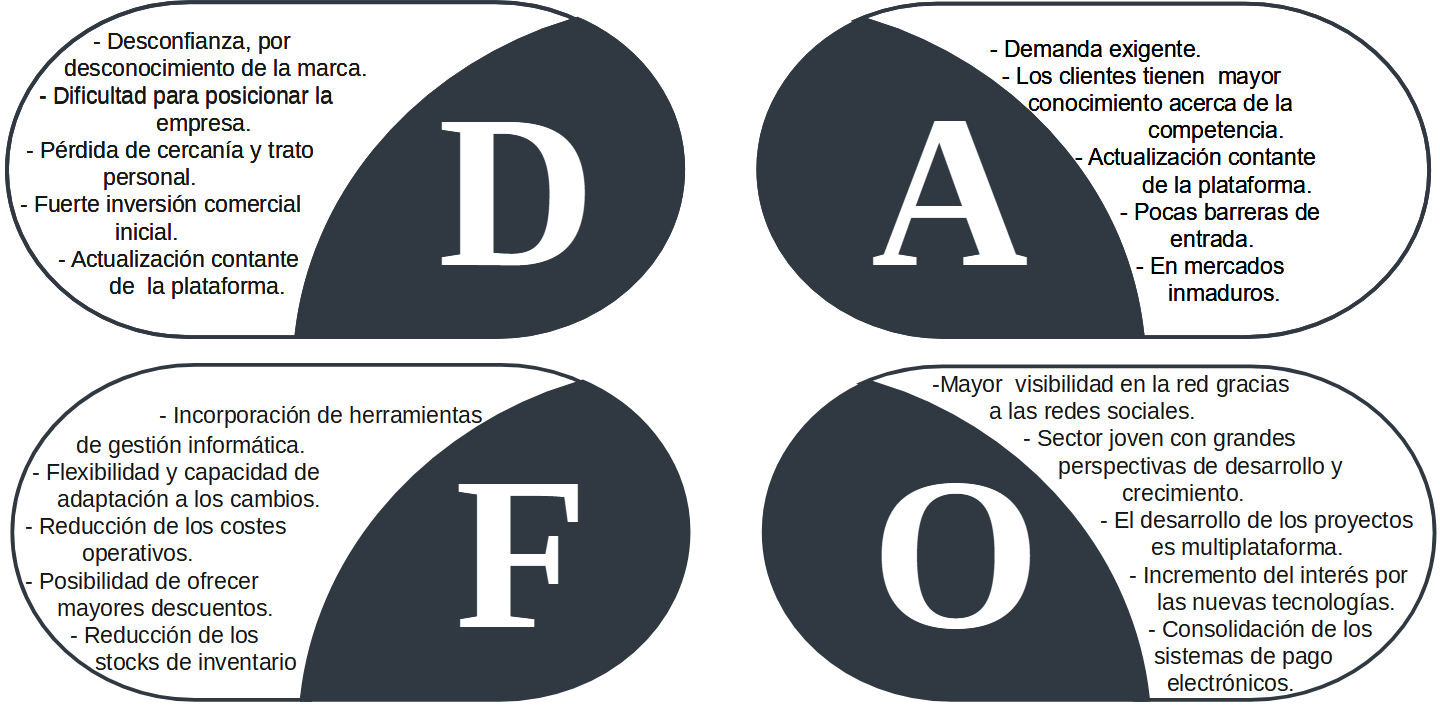
\includegraphics[scale = 0.39]{imagenes/DAFO.png}
\renewcommand{\figurename}{DAFO}
\renewcommand{\thefigure}{}
\caption{\textit{Debilidades, Amenazas, Fortalezas, Oportunidades}}
\end{figure}
\begin{figure}[h]
\centering
\renewcommand{\figurename}{CAME}

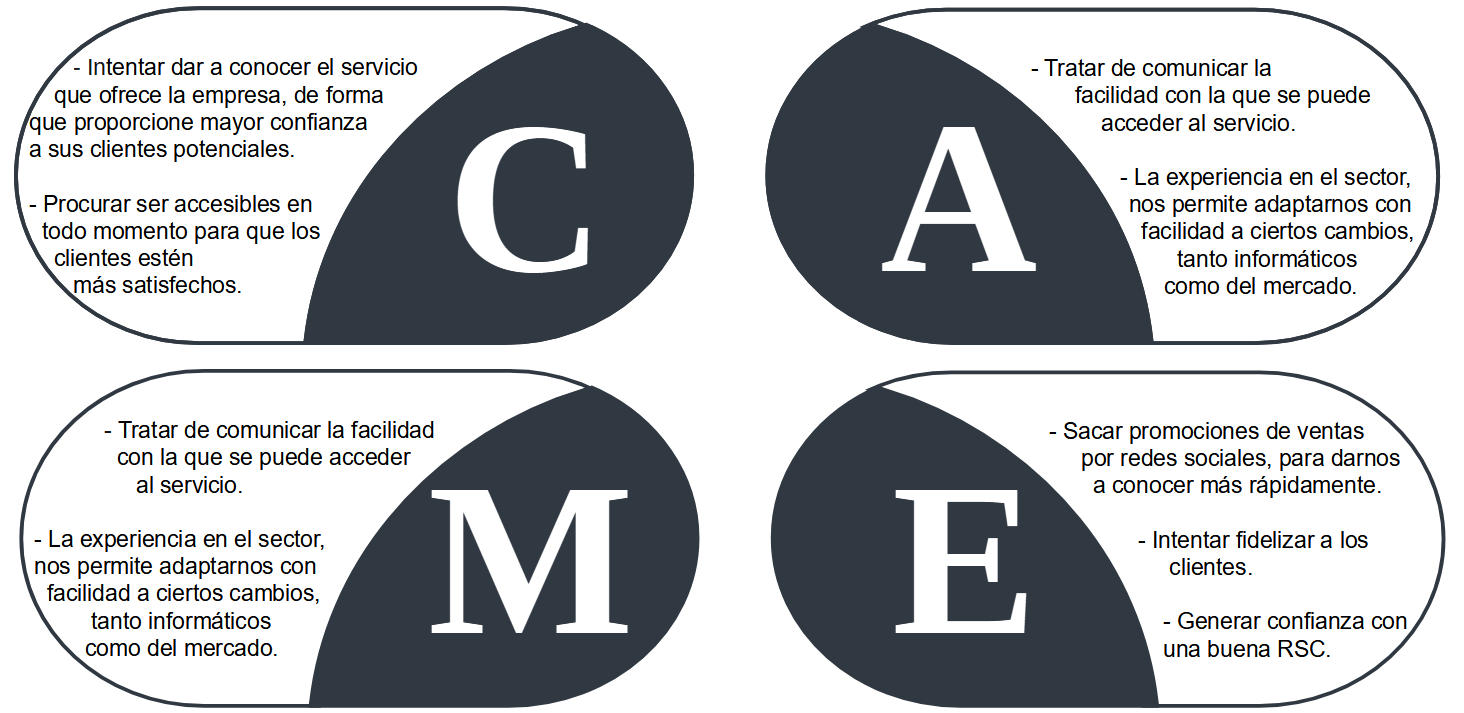
\includegraphics[scale = 0.39]{imagenes/CAME.png}
\renewcommand{\thefigure}{}
\caption{\textit{Corregir las debilidades internas, Afrontar las amenazas externas, Mantener las fortalezas internas, Explotar las oportunidades externas}}
\end{figure}
\newpage
\section{Localización} 
%
%
% Falta poner donde vamos a trabajar físicamente y hay que poner un servidor mas económico
%
%
%
Al ser una empresa online no será necesario un gran local. Tan solo necesitaremos una oficina física con una buena conexión a internet. Para cumplir esto se ha elegido un edificio junto a la Universidad, lo cual pondrá a la empresa cerca de los clientes de forma física.\\
\begin{figure}[h]
\centering


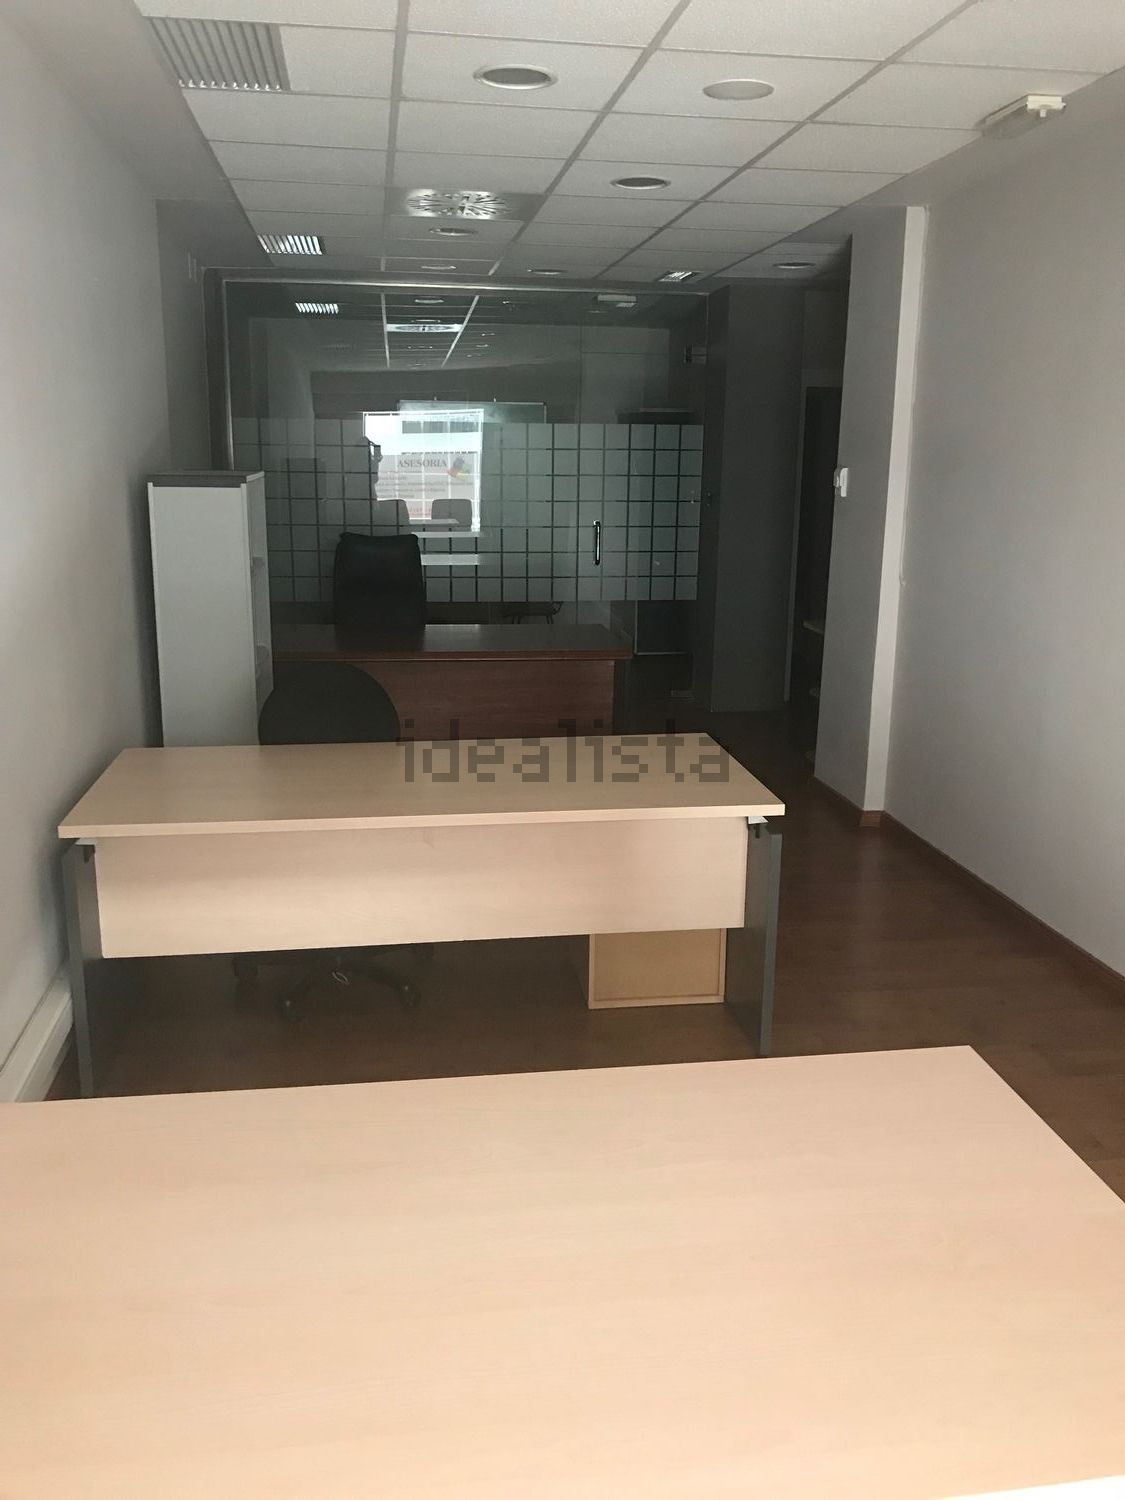
\includegraphics[scale = 0.2]{imagenes/oficina.jpg}
\renewcommand{\figurename}{Imagen}
\renewcommand{\thefigure}{}
\caption{\textit{Ejemplo de la oficina elegida}}
\renewcommand{\figurename}{Fuente}
\caption{Idealista}
\end{figure}
\\
El coste del local ascenderá a 275 euros al mes, lo cual reducirá los costes en gran medida pero, en cambio, será necesario un servidor.
El servidor será contratado en Amazon AWS, por un precio de 0,08 euros por GB al mes. A esto habrá que sumarle el coste de un dominio, el cual asciende a 15 euros anuales. También hay que tener en cuenta las operaciones de entrada y salida (IOPS) del servidor y el ancho
de banda. El servicio de AWS ofrece 1.000 IOPS gratuitas, pero podríamos aumentar a 3.000 IOPS y adquirir un ancho de banda de 300 MB/s. El coste mensual ascendería a 889 euros.
\newpage
A esto habría que añadirle un servicio de seguridad. Cloudflare tiene un servicio básico gratuito para evitar los principales ataques, por lo que no aumentaría el presupuesto.
\\
Para reducir el precio del servidor se creará una red \textit{Peer-to-peer}, comunmente conocida como P2P.\\Esta red permite a los usuarios convertirse en nodos de la propia conexión y compartir a la vez que descargan contenido. De esta forma se podrá ofrecer descuentos para convertirse en nodo y reduciendo el coste del servidor. Esto repercutirá positivamente en la empresa de dos maneras, primero permitiendo bajar el precio sin incurrir en pérdidas y, al mismo tiempo, reduciendo los costes fijos. 
\begin{figure}[h]
\centering
\renewcommand{\figurename}{Imagen}

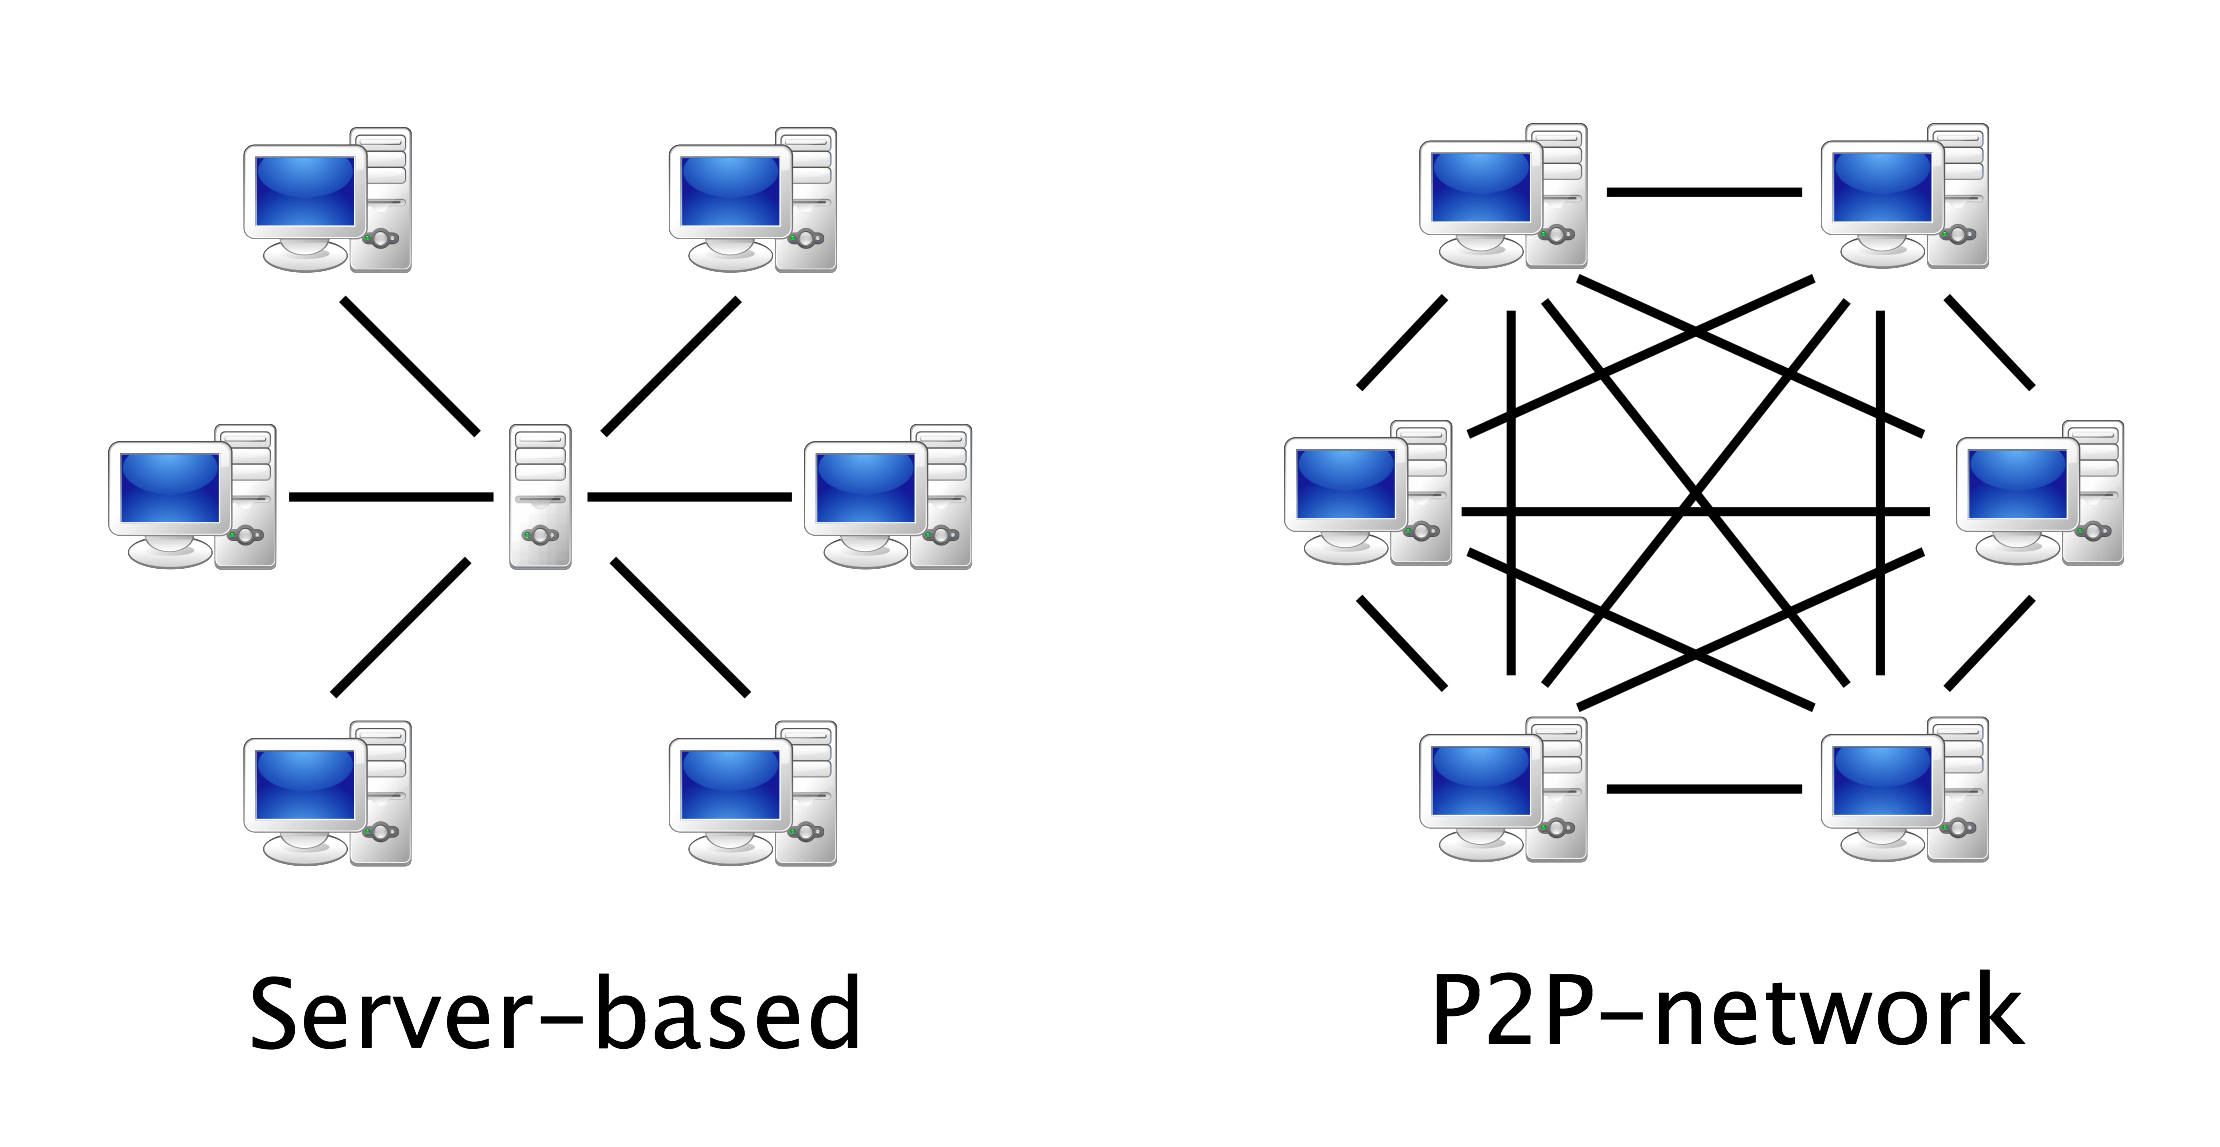
\includegraphics[scale = 0.1]{imagenes/p2p.jpg}
\renewcommand{\thefigure}{}
\caption{\textit{Ejemplo de comparación entre una conexión clásica con servidor y una conexión P2P}}
\end{figure}
\\\\
El uso de esta red está directamente relacionado con la cantidad de usuarios-nodos de los que se disponga. Por lo que, cuanto mayor sea la empresa, menor será el coste de servidor.


\setcounter{chapter}{4} %Cambiamos el numero del capitulo
\chapter*{Tema 4. El marketing}
\addcontentsline{toc}{chapter}{Tema 4. El marketing}
\setcounter{section}{0}
\section{Posicionamiento a alzanzar en el mercado}
\subsection{Calidad del producto}
El servicio que ofrecerá la empresa será de alta calidad, pero sin llegar a ser un producto de lujo. Esta empresa tratará siempre de ser eficaz y muy limpia y además contará con una interfaz que facilite su uso.
\subsection{Precio}
Tendrá un precio medio-bajo para llegar al máximo número de personas pero manteniendo la calidad del servicio. Lo que supondrá un precio de entre 4€ - 10€ mensuales.
\subsection{Valor percibido}
Las campañas de marketing irán orientadas a demostrar que el servicio tiene alta calidad, fácil acceso y además a un precio razonable. Además, sobre todo al principio, para darnos a conocer, queremos que los consumidores perciban a la empresa como una amplia gama de libros electrónicos para todos los gustos, bajo demanda y con recomendaciones personalizadas a cada usuario.
\subsection{Mapa de posicionamiento}
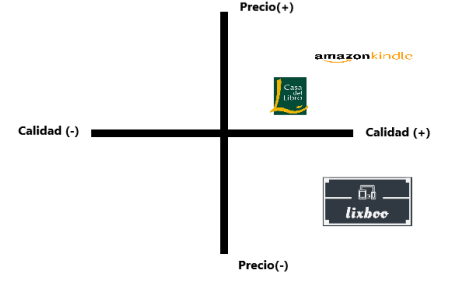
\includegraphics[scale = 0.9]{imagenes/mapa de posicionamiento.png}
\section{Producto}
\subsection{Niveles del producto}
Este apartado se divide en tres niveles:
\begin{itemize}
\item Producto básico, en este apartado se ha analizado la necesidad del servicio que ofrece la empresa, por lo que, se puede decir que dicha necesidad será la posibilidad de leer libros desde cualquier parte, sin que haga falta tener todos estos de forma física.
\item Producto formal, sobre las características tangibles que se pueden observar, se ha considerado que, al tratarse de un servicio, hay algunos aspectos que no se pueden controlar. Como por ejemplo: al ser un servicio bajo demanda, la cantidad es elegida por el usuario. Igualmente la calidad del producto depende en gran medida del usuario, ya que, aun ofreciendo una gran calidad, esta podría verse mermada por el dispositivo usado.
\item Producto ampliado. A la suscripción se añadirán ventajas adicionales, por ejemplo, un descuento si la suscripción es anual, derecho a voto para elegir libros a añadir al catálogo o, en algunos casos, el préstamo gratuito de un libro electrónico para leer.
\end{itemize}
\subsection{Tipos de producto}
La empresa va a ofrecer un producto intangible, es decir, un servicio, ya que la biblioteca en línea se encuentra en una página web. Por otro lado, contará como un producto sustitutivo respecto a los libros físicos, los cuales son más caros y menos accesibles.
\subsection{Ciclo de vida del producto}
El servicio que ofrece la empresa no es nuevo. Al hacer el estudio del mercado, se pudó observar que el servicio se encuentra ya en la fase de madurez, debido a que, posiblemente, haya llegado a su tope de ventas y su curva de crecimiento se haya aplanado. En consecuencia, la empresa quiere anticiparse a la fase de declive y quiere relanzar ese mismo producto pero con innovaciones, como pueden ser las recomendaciones personalizadas.
\subsection{Estrategias sobre el producto}
\begin{wrapfigure}{r}{0.25\textwidth}

\includegraphics[width=0.75\linewidth]{imagenes/lixboo.png}
\caption{Marca de la empresa}
\end{wrapfigure}
La principal diferencia del producto de la empresa respecto a los de la competencia es la posibilidad de crear una lista de sugerencias para el cliente, teniendo en cuenta los libros que ha estado leyendo hasta el momento y sus gustos para, así, crear un modelo de usuario a comparar con los demás.
\clearpage %La figura no mueve la parte posterior
Su nombre, Lixboo, se crea mediante la combinación libro y book (libro en inglés). El logo representa los dispositivos desde los que se puede leer.
Por otro lado, aunque no aparezca en el logo, el eslogan de la empresa será: “Lixboo en línea”.
\section{Precio}
\subsection{Criterio de fijación del precio}
Para fijar el precio se tomarán como referencia tanto los costes (acuerdos con las editoriales, mantenimiento de la web y servidores, etc), la competencia (se comparará con otros servicios bajo demanda) y los consumidores (se tiene que abarcar al mayor número de personas posible pero no fijar un precio por debajo del valor percibido). Después de tener en cuenta estos tres aspectos, se ha decidido que el precio oscila entre 25€ y 30€ al mes.
\subsection{Estrategia de penetración}
En un principio, la idea de la empresa es fijar un precio por valor del 50\% los 6 primeros meses después del lanzamiento para llegar y fidelizar a más gente.
\subsection{Estrategia sobre precios}
Se intentará utilizar algunas estrategias sobre el precio como puede ser:
\begin{itemize}
\item Precios psicológicos, es decir, poner precios que terminan en 95 o 99, preferiblemente que acaben en impar.
\item Discriminación de precios, en el caso de que el consumidor sea estudiante o de algún otro colectivo se podrían realizar descuentos para estos en concreto.
\item Precio paquete, la empresa también ofrecerá paquetes en el que un grupo de personas contraten nuestro servicio y resulte más económico.
\end{itemize}

\section{Actividades de promoción} 
%%%%%%%%%%%%%%%%%%%%%%%%%%%%%%%%%%%%%%%%%%%%%%%%%%%%%%%%%%%%%%%%
%%%%%%%%%%%%%%%%%%  HAY QUE MIRAR LOS PRECIOS DEL NUEVO SERVIDOR...
%%%%%%%%%%%%%%%%%%%%%%%%%%%%%%%%%%%%%%%%%%%%%%%%%%%%%%%%%%%%%%%%
La mejor manera de promocionar la empresa será una combinación en distintos ámbitos.
Algunas de las medidas serían repartir folletos en las facultades de letras de distintas ciudades, pactar colaboraciones con creadores de contenido literarios en redes sociales y enviar publicidad a través del correo electrónico con ofertas personalizadas.
\\Para la fidelización de los clientes, se podrían ofrecer descuentos por mantener la suscripción, merchandising de la empresa (Bolígrafos y cuadernos…).
\\Para mejorar la imagen corporativa de la empresa y hacerla conocer, se puede llevar a cabo un concurso. Como ejemplo, un concurso de novelas, siendo la ganadora editada para formato electrónico de manera gratuita y publicada en nuestra página.
Estas actividades de promoción supondrán una serie de costes, que se podrían resumir en:
\begin{itemize}
\item El coste de imprimir 20.000 folletos sería 318 €.
\item El coste del reparto de folletos sería, aproximadamente, 30€ cada 1.000 unidades, por lo que repartir los folletos costaría 600€.
\item Así mismo, una colaboración pagada con un creador de contenido en redes sociales costaría, aproximadamente, 100-150€. Calculando al alza y contando con 5 creadores de contenido, esto supondría 750€.
\end{itemize}
Así pues, el coste total de la promoción ascendería a 4.387€.
\\
En el área de promoción se incluirá, pasado un tiempo, la posibilidad de convertirse en nodo de la red, a cambio de un descuento dependiente de la cantidad de datos compartidos. 




\section{Canal de distribución}
La estructura del canal de distribución, tal y como se explica en el esquema siguiente, se basa en un canal indirecto corto, ya que, los libros los comprará la empresa 
\begin{wrapfigure}{l}{0.25\textwidth}
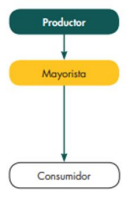
\includegraphics[width=0.9\linewidth]{imagenes/canales de distribucion.png} 
\caption{Canales de distribución}
\end{wrapfigure}
  directamente a las editoriales es decir, a los fabricantes. Por lo tanto, la empresa contará con un canal de distribución directo, en forma digital, mediante internet.

\clearpage %La figura no mueve atención al cliente
\newpage

\section{Atención al cliente}
\subsection{Organización}
Una única persona se dedicará a la atención al cliente. Responderá en horario comercial al número de teléfono propio y al correo electrónico. Las llamadas y los correos se registrarán en una base de datos para aplicar las mejoras sugeridas directa o indirectamente por estos medios o por una pestaña de la web para esta finalidad.
\subsection{Gestión de reclamaciones y sugerencias}
Las reclamaciones se gestionarán de la forma más cordial posible y guiando al cliente para solucionar el problema si es por su parte o con una pequeña compensación si ha sido un error de la empresa, como por ejemplo con un mes gratis.
\\Habrá un departamento orientado a la mejora del servicio que será el que lea las sugerencias y valorará si hacerlas y cómo hacerlas.


\subsection{Servicio post-venta y garantía}
En cuanto a la garantía, siempre se tratará de ofrecer la mejor calidad del servicio, es decir, se contará con un profesional de HTML y Marketing Digital, que será contratado para realizar la página web donde ofrecerá el servicio.
Por otro lado, el servicio post-venta está directamente ligado con la gestión de reclamaciones y sugerencias.
\subsection{Encuestas de satisfacción}
A las 5 descargas de libros podría saltar una pequeña encuesta en la que se pueda valorar opcionalmente el servicio y aportar alguna sugerencia. Algunos de los aspectos que se podrían valorar, podrían ser: la fluidez de la interfaz, la distribución de elementos en la web o la oferta de libros de los que disponga el servicio.
\subsection{Orientación hacia el cliente}
Se transmitirá la filosofía de orientación hacia el cliente en nuestros departamentos por parte de algún cargo intermedio con experiencia en este tipo de puestos. Será importante tener al cliente satisfecho para fidelizarlo y que recomiende la empresa.
\setcounter{chapter}{5} %Cambiamos el numero del capitulo
\chapter*{Tema 5. Recursos Humanos}
\setcounter{section}{0}
\section{Dirección y liderazgo}
La empresa estará compuesta por dos socios: María Herrero y Héctor Carcasona. Ambos dirigirán la empresa, de forma que en la toma de decisiones, estas deberán pasar bajo la supervisión de estos socios.
\section{Motivación laboral}
Con la posibilidad del teletrabajo, no será necesario preocuparse de algunos aspectos de seguridad de las empresas convencionales (como las referidas al edificio).
Además, la empresa tratará de motivar a sus trabajadores de forma intrínseca, ya que, además de valorar el trabajo que hace cada uno de ellos, intentará que exista variedad para evitar tareas monótonas como la conciliación bancaria o con que los trabajadores cuenten con la autonomía suficiente como para tomar decisiones acerca de cómo realizar el trabajo.
\section{Organigrama de la empresa}
En la dirección aparece nuestro directivo, en el departamento de servicio se contará con un empleado contratado para realizar la página web con la que la empresa prestara su servicio. De la parte económica se encargarán María y Héctor.\\
Por otro lado, se realizará subcontratación de la contabilidad y fiscalidad de la empresa. Y además se contratarán a dos empleados más, uno para el departamento de marketing y otro empleado para la parte de la página web.

\begin{figure}[h]
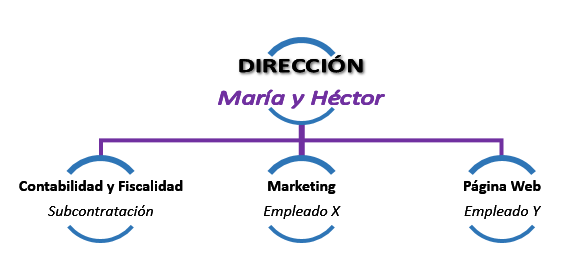
\includegraphics[scale = 0.8]{imagenes/organigrama.png}
\centering\renewcommand{\thefigure}{}
\caption{Organizagrama de Lixboo.}
\end{figure}

\section{Contrataciones}
En un primer momento, la empresa va a necesitar únicamente a dos empleado, uno de ellos  se hará cargo de la página web. Por lo tanto, habría que contratar a alguien con experiencia en HTML, CSS e incluso con conocimientos en Marketing Digital. \\La idea de la empresa, es contratar a esta persona con un contrato indefinido, pero con un periodo de prueba de 4 meses. Por otro lado, se contará con un experto en marketing, para poder planificar toda las campañas publicitarias que se van a llevar a cabo, además de tomar decisiones acerca de las promociones etc, que ofrecerá la empresa.
\\El convenio colectivo al que va a pertenecer estos contratos es al convenio colectivo de la industria, la tecnología y los servicios (siderometalúrgica). La categoría profesional será la 2, ya que, lo agrupan según convenio: Técnico no titulado, Técnico, Jefe de 1.ª administrativo y Delineante Proyectista.
Este trabajador contará con un salario de 15.583 € según las tablas salariales de ese convenio.

\setcounter{chapter}{6}
\chapter*{Tema 6. Forma jurídica}
\setcounter{section}{0}
\section{Sociedad limitada}
Se ha elegido la sociedad limitada como forma jurídica para la empresa. Esta forma ofrece distintas ventajas, siendo las principales:
\begin{itemize}
    \item Responsabilidad limitada a la aportación
    \item División de la empresa en participaciones
    \item Capital mínimo para constituir la sociedad
\end{itemize}
La sociedad limitada es una forma más segura que la sociedad anónima, ya que tu responsabilidad está limitada a la aportación que realices, por lo que tus bienes privados están seguros.\\\\ Al ser la empresa dividida en participaciones, se mantiene un control sobre ella, aunque limitando las opciones para nuevos inversores. \\\\
A parte de esto, el capital mínimo son tan solo 3000 €, muy alejados de los 60.000 de las sociedades anónimas. 

\section{Socios de la empresa}
En la empresa habrá dos socios, María y Héctor. Ambos se ocuparán de labores de la empresa y tendrán un porcentaje de participación equivalente a la inversión realizada. \\\\La empresa no está cerrada a la entrada de nuevos socios, siempre asegurando que el porcentaje de acciones de los socios fundadores sea, como mínimo, 50 \% + una acción.

\section {Capital disponible}
La suma del capital disponible entre ambos socios será de 60.000 €, habiendo aportado ambos 30.000 €. Este capital es más que suficiente para la puesta en marcha de la empresa y su sustento durante, al menos, un ejercicio. 
\section{Relación entre los socios}
La relación entre los socios es una férrea amistad con la misma visión en cuanto al camino que la empresa debe seguir, lo cual asegurará que haya las mínimas discrepancias en la toma de decisiones. 
\section{Ayudas disponibles}
La empresa y los socios tendrán acceso a varias ayudas, entre ellas: 
\begin{itemize}
    \item Tarifa plana de 60 € al mes como cuota de autónomos durante el primer año
    \item El 'Proyecto SURGE' otorga subvenciones a pequeñas empresas si se contrata en municipios de menos de 30.000 personas.
    \item Subvenciones por la contratación de empleados a cuenta ajena
\end{itemize}
\setcounter{chapter}{7} %Cambiamos el numero del capitulo
\chapter*{Tema 7. El plan de producción}
\setcounter{section}{0}
\section{El plan de producción}
\subsection{Listado de bienes que vamos a necesitar}
\begin{itemize}
    \item Local (calefacción, electricidad, agua, alquiler...)
    \item Escritorios para ambos socios y también para los empleados (3)
    \item Ordenadores con pantalla, ratón y teclado
    \item Sillas Ergonómicas
\end{itemize}
\subsection{Listado de servicios que vamos a necesitar}
\begin{itemize}
    \item Servidor
    \item Dominio
    %%%%%%%%%%%%%%%%%%%%%%%%
    %%%%%%%%%%%%%%%%%%PENSAREMOS MAS OTRO DIA
%%%%%%%%%%%%%%%%%%%%%%%%%    
\end{itemize}
\subsection{Listado de servicios que vamos a ofrecer}
\begin{itemize}
    \item Libros bajo demanda
    \item Recomendaciones de lectura
    \item Tratamiento personalizado
    
\end{itemize}
\subsection{Revisión del personal}
\begin{itemize}
    \item Socios (Héctor y María)
    \item Empleado para el departamento de marketing
    \item Empleado para el departamento web
\end{itemize}
\newpage
\section{Costes fijos y variables}

\begin{figure}[h]
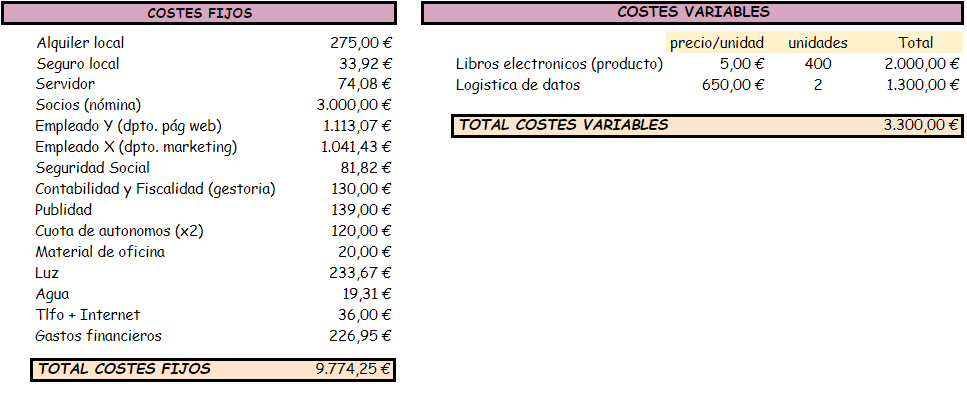
\includegraphics[scale = 0.55]{CostesFVBUENO.png}
\centering\renewcommand{\thefigure}{}
\newpage
\caption{Costes fijos y variables del primer mes.}
\end{figure}
Ahora vamos a calcular el punto muerto a partir de esta fórmula: 
\\\[ Q*= \frac{CF}{(P-CVU)}\]
\\\[ Q*= \frac{9.774,25}{(30-5)}\]
\\\[390,91 = \frac{9.774,25}{(30-5)}\]

El punto muerto o umbral de rentabilidad de Lixboo oscilará en torno 391 unidades. Es decir, que la empresa tendrá que vender cada mes 391 suscripciones, para poder obtener algo de beneficio.
\newpage

\setcounter{chapter}{8} %Cambiamos el numero del capitulo
\chapter*{Tema 8. Inversión y Financiación}
\setcounter{section}{0}
\section{Inversiones}
\begin{figure}[h]
%%%%%%%%%%%%%%%%%%%%%%%%%%%%%%%%%%%%%%%%%%%
%%%%%%%%%%%AÑADIR DOMINIO Y SERVIDOR Y CUATRO ESCRITORIOS
%%%%%%%%%%%%%%%%%%%%%%%%%%%%%%%%%%%%%%

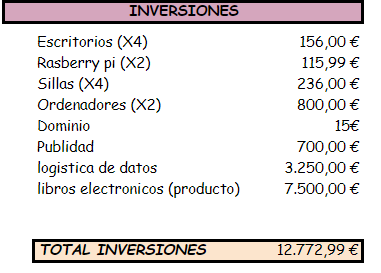
\includegraphics[scale = 0.8]{inversiones.png}
\centering
\caption{Inversiones a realizar el primer mes.}


\end{figure}
No será necesario invertir ni en inmuebles ni en servidor, ya que la empresa alquilará ambas.\\Los escritorios y el mobiliario serán comprados en Ikea, mientras que los ordenadores serán montados a piezas en PCComponentes.
\newpage
\chapter*{Tema 9: Análisis contable y financiero}
\addcontentsline{toc}{chapter}{Tema 9: Análisis contable y financiero}
\section{Plan de tesorería}
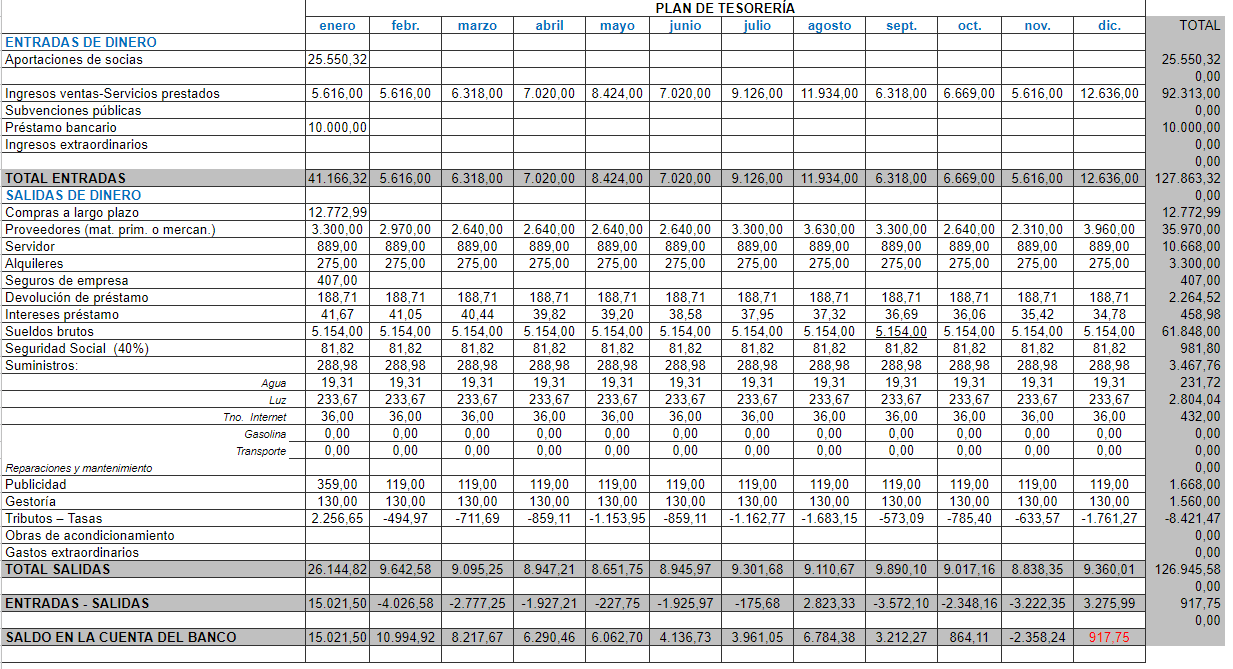
\includegraphics[scale = 0.53]{planTesoreria.png}


\section{Cuenta de resultados}
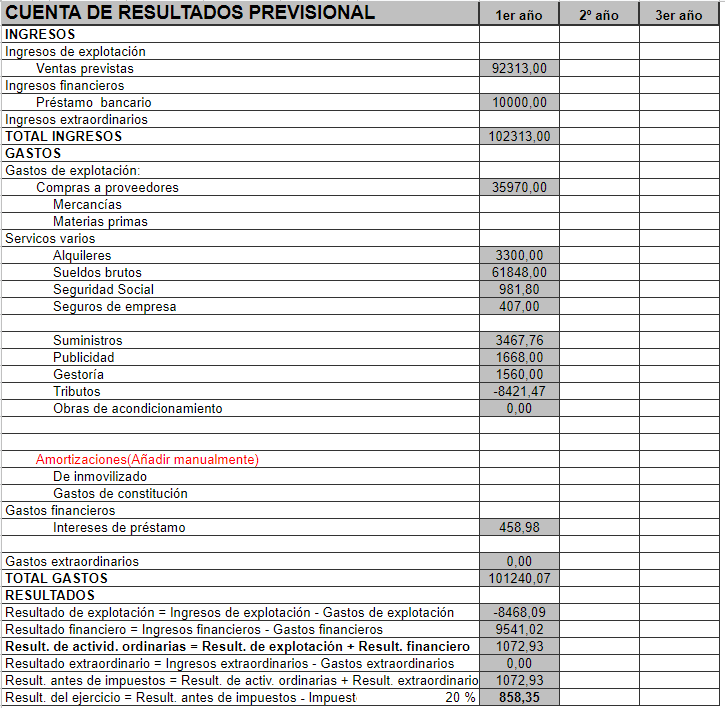
\includegraphics[scale = 0.65]{cuentaResultados.png}

\newpage
\section{Balance de situación}
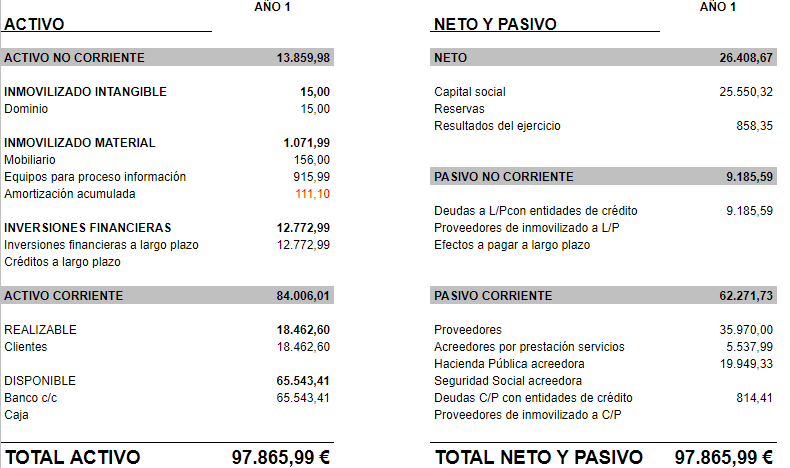
\includegraphics[scale = 0.7]{balanceSituacion.png}



\chapter*{ANEXOS}
\addcontentsline{toc}{chapter}{Anexos}
A continuación se añaden los anexos del plan de empresa: La encuesta y la amortización del crédito pedido 
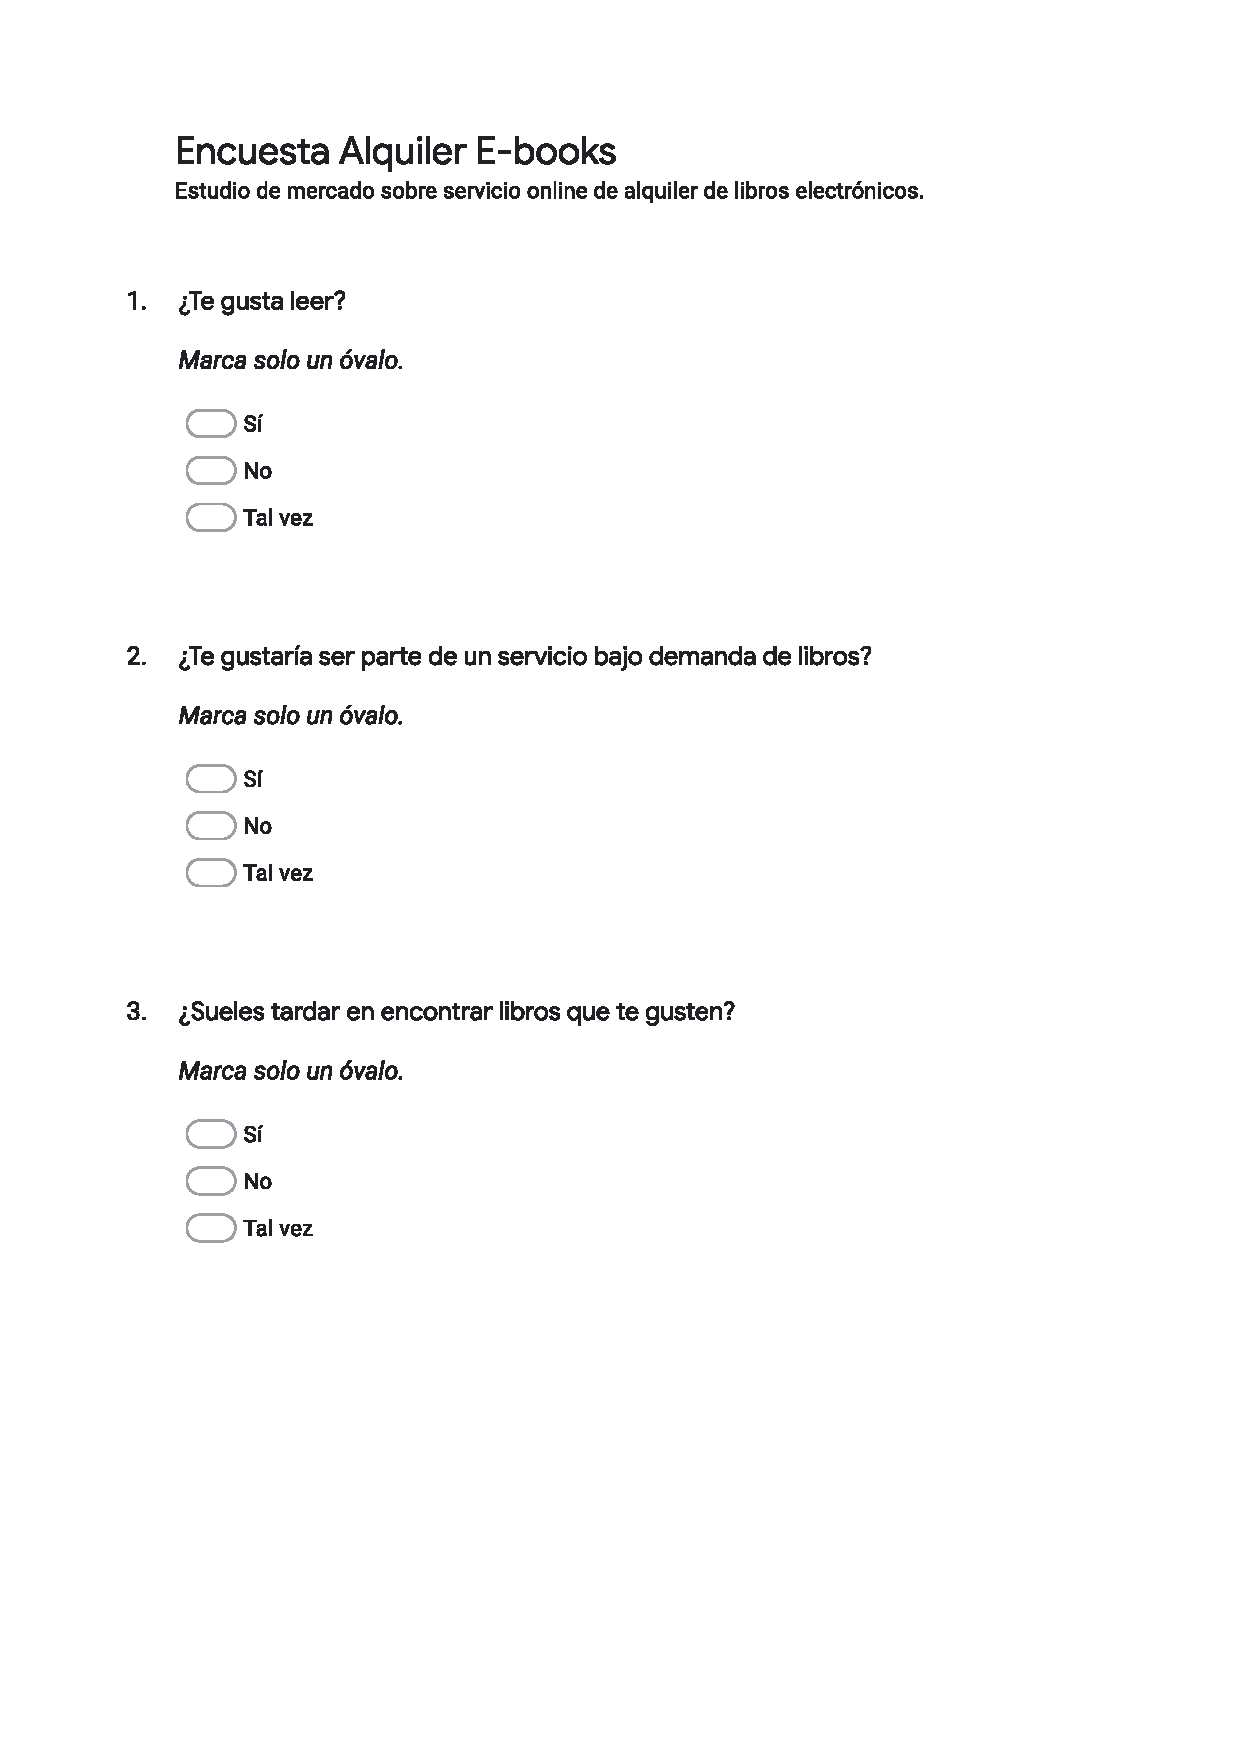
\includepdf[pages=1,pagecommand=\section*{Encuesta}, offset=0 -3cm]{encuesta.pdf}
\includepdf[pages=2]{encuesta.pdf}
%includepdf[pages=-]{NuevoCredito.zip}
\end{document}
